\documentclass[12pt]{report}
\usepackage{amsmath}
\usepackage{amsfonts}
\usepackage{hyperref}
\usepackage{tikz}
\usetikzlibrary{arrows.meta}
\usepackage{graphicx}
\usepackage{caption}
\usepackage{subcaption}
\usepackage{listings}
\setlength{\oddsidemargin}{0.5in}
\setlength{\evensidemargin}{0.5in}
\setlength{\textwidth}{6.0in}
\setlength{\topmargin}{.75in}
\setlength{\textheight}{8.6in}

\newcommand{\e}{\vec e}
\newcommand{\citeneeded}{\footnote{\textit{citation needed}}}
\newcommand{\half}{\frac{1}{2}}
\newcommand{\codeexample}[1]{
    \section{\texttt{#1}}
    \lstinputlisting[language=C++]{../code/cpp_code/#1}
}

% Modified by S. Aubin for the class of 2019 Physics theses

%
% This is a LaTeX template for an undergraduate honors or
%   senior thesis in physics at William & Mary. Created from
%   several theses from previous students of D.S. Armstrong,
%   pared down to bare bones.
%
%   you will need this present file (thesis_template.tex)
%   as well as the file  figure1.eps  to make the whole thing
%   (the latter is just an encapsulated postscript figure)
%     For simplicity, we don't use bibtex here; experts can choose
%   to use that more powerful way of dealing with citations.
%
%   To compile it, do:
% > pdflatex thesis_template.tex
% > pdflatex thesis_template.tex  (yes, you need to do it twice to
%                                  fill in the list of tables, figures
%                                  and references).



\begin{document}
\setlength{\baselineskip}{24pt}
\begin{titlepage}
\LARGE
\begin{center}
    {\bf Topology of the $O(3)$ non-linear sigma model under the gradient flow}\\[2.3cm]

\normalsize
A thesis submitted in partial fulfillment of the requirement \\
for the degree of Bachelor of Science with Honors in \\
Physics from the College of William and Mary in Virginia,\\[0.5cm]
by\\[0.5cm]
Stuart Thomas \\[2.5cm]
\end{center}
\normalsize
\begin{flushright}
%\hfill Accepted for Honors \\[.5cm]
\hfill \hrulefill \\
\hfill \hfill Advisor: Prof. Christopher J. Monahan\\[.6cm]
\hfill \hrulefill \\Prof. Todd Averett \\[.6cm]
\hfill \hrulefill \\Prof. Andreas Stathopoulos \\[.6cm]
\end{flushright}
\begin{center}
Williamsburg, Virginia\\
May 2021
\end{center}
\end{titlepage}

\setlength{\topmargin}{0.0in}

\pagenumbering{roman}
\tableofcontents
\chapter*{Acknowledgments}
\addcontentsline{toc}{chapter}{Acknowledgments}
\paragraph
\indent I would like to thank lots of people, and this is where
I will do it...


\listoffigures
\addcontentsline{toc}{chapter}{List of Figures}
\listoftables
\addcontentsline{toc}{chapter}{List of Tables}

\begin{abstract}
\setcounter{page}{5}
\addcontentsline{toc}{chapter}{Abstract}
\paragraph
\indent \textit{Abstract}

\end{abstract}

\pagenumbering{arabic}
\chapter{Introduction}

Quantum field theory (QFT) is an extraordinarily successful framework which can be applied to a range of physical phenomena. Paired with the Standard Model, QFT provides the prevailing basis for all small-scale physics (that is, where general relativity does not apply) and is the fundamental tool for studying particle physics. In condensed matter physics, effective field theories model emergent effects such as phonons and quasiparticles. Compared to experiment, QFT is remarkably accurate, famously matching the experimental value for the electron $g$-factor to eight significant figures.\cite{weisskopf1981} 

However, this power comes at a cost: the study of quantum fields is rife with infinities. A na\"ive treatment of quantum field theory produces divergent values for physical quantities, a clearly impossible result. Since the 1950s, this issue has been resolved for a large number of models--- most notably quantum electrodynamics--- through perturbation theory and the so-called \textit{renormalization group}. However, the technique fails with perturbatively nonrenormalizable theories. 

One such example is the \textit{non-linear sigma model}, a prototypical theory in both condensed matter and particle physics. In solid-state systems, this model describes Heisenberg ferromagnets and in nuclear physics, it acts as a prototype for quantum chromodynamics (QCD), exhibiting characteristic features such as a mass gap and asymptotic freedom. \citeneeded

In this study, we specifically consider the $O(3)$ non-linear sigma model in $1+1$ dimensions (one dimension of space, one dimension of time). This theory exhibits topological properties such as \textit{instantons}, or classical field solutions at local minima of the action.



Since the non-linear sigma model cannot be renormalized perturbatively, we cannot study these topological effects with normal perturbative techniques. An alternative solution is placing the field on a discretized lattice, a technique originally used for quantum chromodynamics. In this scenario, field configurations become computationally calculable. This process introduces an nonphysical length scale $a$, the lattice spacing. Therefore, we expect any physical result to converge in the continuum limit, i.e. when $a\rightarrow 0$. However, this is not always the case as observables mix on the lattice, leading to divergences. As an example, states of definite angular momentum mix when discretized, a clear violation of the angular momentum commutation relations. 


The gradient flow is a technique designed to remove these divergences. By dampening high-momentum fluctuations, the gradient flow reduces power-divergent mixing and make observables finite on the lattice.\cite{monahan2016} In quantum chromodynamics, previous studies have verified the ability of the gradient flow to make observables finite\citeneeded. Due to its success in QCD, there has been interest in using the gradient flow to finitize the topological susceptibility in the 1+1 $O(3)$ non-linear sigma model.\cite{bietenholz2018}.

%goals here

\section{Method Overview}

To numerically study the topological qualities of the non-linear sigma model, we first implement a Markov Chain Monte Carlo simulation. We initially construct a proof-of-concept Python program that models the simpler $\phi^4$ model (see Sec.~\ref{sec:phi4}). After comparing with existing literature, we transition to a C++ simulation for efficiency, implementing the non-linear sigma model in larger lattices. Since the gradient flow has no exact solution in the non-linear sigma model, we implement a numerical solution using a fourth-order Runge-Kutta approximation. By applying the gradient flow to every configuration in the sample, we can measure its effect on the topological charge and susceptibility.

\section{Conventions}
\begin{itemize}
    \item Throughout this paper, we use natural units, i.e. $\hbar = 1$ and $c=1$.
    \item We use Einstein summation notation, an implicit sum over repeated spacetime indices. For example, if $x^\mu$ is a spacetime four-vector and $x_\mu$ is its covariant form, the term
        \begin{align*}
            x^\mu x_\mu &= \sum^4_{\mu=0} x^\mu x_\mu \\
            &= x_0^2-x_1^2-x_2^2-x_3^2.
        \end{align*}
\end{itemize}

%\section{Main Experimental Goal}

\chapter{Theory}

This thesis incorporates two main bodies of knowledge: quantum field theory and statistical simulation. Through the path integral formulation of quantum field theory, we are able to describe the physics of the former with the established mathematics of the latter.

\section{Quantum Field Theory}


In this section we outline a rough description of quantum field theory. A full introduction is beyond the scope of this paper, however we do assume knowledge of nonrelativistic quantum mechanics and classical field theory.

The fundamental hypothesis of quantum field theory (QFT) describes particles as discrete packets of energy on a quantum field. But what is a quantum field? Like in classical mechanics, a field is a function of spacetime with some mathematical object assigned to each point in space and time. In the case of the electric field, this object is a three-dimensional vector, while the electric potential is a scalar field. Classical and quantum fields have Lagrangians which define how they evolve in time. What differentiates a quantum field from a classical field is superposition: where classical fields have a definite configuration, quantum fields exist in a superposition of all possible configurations. It is possible---though nontrivial and outside the scope of this description--- to motivate the appearance of discrete particles from this superposition.

This general description allows QFT to easily incorporate special relativity. By ensuring that the Lagrangian of a theory is invariant under Lorentz transformations, we can ensure that the theory is physical. % is this enough?

Though most introductions to QFT use the ``second quantization,'' we will use a alternative formulation known as the path integral formulation (for a similar introduction see Zee's textbook \cite{zee2010}).
 
\subsection{Path Integral Formulation}
\label{sec:pathintegral}

As stated above, we can model a quantum field theory as a superposition of all possible classical fields. Like single-particle quantum mechanics, each configuration has a probability amplitude. To measure expectation values of observables, we simply take an average over all configurations weighted by this complex amplitude. We can formalize this notion using the fundamental formula\footnote{Since this study concerns vacua, we do not include a source term.}
\begin{equation}
    \label{eq:pathintegral}
    \langle \hat O \rangle = \frac{1}{Z} \int \mathcal{D}\phi \: \hat O [\phi]\; e^{iS[\phi]}
\end{equation}
% not sure if the semicolons is good form
where $\langle \hat O \rangle$ is the expectation value of an arbitrary operator $\hat O$; $Z$ is a normalization constant; $S$ is the action functional, defined from the field's Lagrangian; and $\int \mathcal{D}\phi$ represents the eponymous path integral. Though it is possible to define this integral rigorously, for our purposes we can equate it to a sum over all possible configurations. This form is the quantum analog of the classical principle of least action and reduces to such for large values of the action. For a more pedagogical explanation, see Richard Feynman's lectures on physics.\cite{feynman1963a}

At first glance, Eq.~\ref{eq:pathintegral} is remarkably similar to the statistics of the canonical ensemble. Through this similarity, we will be able to use mathematical tools from statistical mechanics to study quantum field theories. However, the factor of $i$ in the exponent currently prohibits us from making this jump. To remedy this issue, we perform a ``Wick rotation'' which shifts spacetime into Euclidean coordinates. In normal spacetime, defined by the Minkowski metric, the Lorentz-invariant distance is given as
\begin{equation}
    s^2 = x^2_0 - x^2_1- x^2_3- x^2_3
\end{equation}
where $x_0=ct$ and $\vec{x} = (x_1, x_2, x_3)^T$. By redefining the time coordinate of a spacetime point $x$ to be $x_4=ix_0$, we find that the quantity
\begin{equation}
    s_E^2 = x^2_1+ x^2_3+ x^2_3 + x^2_4,
\end{equation}
is equivalently Lorentz invariant, which is representative of a four-dimensional Euclidean space. Furthermore, we find that
\begin{align}
    d^4x_E &= d^3\vec{x}dx_4 \\
    &= i d^3\vec{x}dx_0 \\
    &= i d^4x. \label{eq:wickdifferential}
\end{align}

We can use this transformation to redefine the Lagrangian $\mathcal{L}$ in Euclidean space as $\mathcal{L}_E$, replacing all $x_0$ with $ix_0$. Since a Lorentz-invariant Lagrangian must include only even powers and derivatives of $x$, the Euclidean Lagrangian remains real. Subsequently, we can define a Euclidean action based on the differential in Eq.~\ref{eq:wickdifferential}:
\begin{align}
    S_E &= \int d^4x_E \mathcal{L}_E \\
    &= i \int d^4x \mathcal{L}_E,
\end{align}
allowing us to redefine the path integral as 
\begin{equation}
    \label{eq:pathintegraleuclidean}
    \langle \hat O \rangle = \frac{1}{Z} \int \mathcal{D}\phi \: \hat O (\phi)\; e^{-S_E[\phi]}.
\end{equation}

By replacing the Minkowski action $S$ with a Euclidean action $S_E$, we have transformed the amplitude $e^{iS}$ to a statistical Boltzmann factor $e^{-S_E}$. This new form will allow us to use statistical techniques to simulate quantum fields.

\subsection{$\phi^4$ model}
\label{sec:phi4}

The simplest interacting field theory is known as the $\phi^4$ model. This theory describes a spin-0 boson and consists of a real scalar field given by the action
\begin{equation}
    \label{eq:phi4 action}
    S[\phi] = \int d^D x \left[ \frac{1}{2}\partial^\mu \phi \partial_\mu\phi - \frac{1}{2} m_0^2 \phi^2 - \frac{\lambda}{4}\phi^4\right].
\end{equation}
The first two terms describe a free relativistic particle of mass $m_0$ while the last term describes an interaction with strength $\lambda$. Note that we have generalized the action for $D$ dimensions. Per Einstein summation notation, there is an implicit sum over spacetime dimensions $\mu\in\{0,1,2,3\}$ indexing the derivative vectors\footnote{This canonical representation of the kinetic term $\frac{1}{2}\partial^\mu\phi\partial_\mu\phi$ is equivalent to $\frac{1}{2}\dot\phi^2-\frac{1}{2}\left(\nabla \phi\right)^2$.}
\begin{align*}
    \partial^\mu &= \left( \frac{\partial}{\partial t}, \frac{\partial}{\partial x},\frac{\partial}{\partial y}, \frac{\partial}{\partial z} \right) \\
    \partial_\mu &= \left( \frac{\partial}{\partial t}, -\frac{\partial}{\partial x}, -\frac{\partial}{\partial y}, -\frac{\partial}{\partial z} \right).
\end{align*}
Following Sec.~\ref{sec:pathintegral}, we calculate the Euclidean action in 1+1 dimensions as 
\begin{equation}
    \label{eq:phi4 euclidean action}
    S_E[\phi] = \int d^2 x_E \left[\frac{1}{2}\left(\partial_t \phi\right) + \frac{1}{2} \left(\partial_x \phi \right) + \frac{1}{2} m_0^2 \phi^2 + \frac{\lambda}{4}\phi^4\right].
\end{equation}
where $\partial_t$ and $\partial_x$ are the two derivatives in 1+1 Euclidean spacetime. 

This field features spontaneous symmetry breaking at a critical value of $m_0^2$. In practice this property causes the field to spontaneously align, similarly to spins aligning in a ferromagnet. The name ``symmetry breaking'' refers to the transformation $\phi\rightarrow-\phi$, which changes the values of observables in the aligned regime but not the disordered regime. These two phases are known as the ``broken'' and ``symmetric'' phases and their transition is well understood.


\subsection{Non-linear sigma model}

The non-linear sigma model (NLSM) is a prototypical theory for many physical phenomena, including applications in string theory. As a simple nonperturbative model, it provides an ideal starting point for lattice QCD studies. Specifically, the NLSM exhibits many properties shared by Yang-Mills gauge theories, such as a mass gap, asymptotic freedom and $O(2)$ renormalizability. Furthermore, it has an exact application to Heisenberg ferromagnets in condensed matter. 

Unlike the $\phi^4$ model, which consists of a real value at each point in spacetime, the $O(3)$ NLSM consists of a 3D unit vector at each point. For this reason, every transformation of the field must be ``norm preserving''. Per its name, the non-linear sigma model features a global symmetry under the 3D orthogonal group $O(3)$. In other words, the theory is invariant under rotating all vectors. To differentiate it from the $\phi^4$ model, we denote the NLSM field as $\e(x)$.

The theory is defined by the Euclidean action 
\begin{equation}
    \label{eq:nlsm euclidean action}
    S_E = \frac{\beta}{2} \int d^Dx \partial^\mu \e \cdot \partial_\mu \e
\end{equation}
subject to the constraint that $\e\cdot\e = 1$. Here, $\beta$ is the inverse coupling.


\section{Markov Chain Monte Carlo}

To accomplish a statistical analysis of quantum fields, we use a Monte Carlo simulation. This method amounts to producing a large number of configurations and calculating statistics on the sample. A brute-force calculation over all possible configurations---as Eq.~\ref{eq:pathintegraleuclidean} suggests--- is clearly infinite and computationally infeasible. However, the exponential nature of the Boltzmann factor dictates that only configurations near the action minimum contribute to observable statistics. Therefore, by selecting a sample of configurations near this minimum, we are able to extract meaningful results with a finite computation.

\subsection{The Markov Chain}
The Markov chain is an effective method to identity these low-action states. Essentially, we begin with a random configuration and then make small adjustments, gradually lowering the action. Starting with a field configuration $\phi_a$, we propose a new field $\phi_b$. The probability of accepting this change, thereby adding the configuration to the chain, is given by the function 
\[P(\phi_a \rightarrow \phi_b).\]



There are four requirements that this function must obey to produce a Boltzmann distribution of samples:
\begin{enumerate}
    \item $P(\phi_a \rightarrow \phi_b)$ must depend only on the configurations $\phi_a$ and $\phi_b$.
    \item The probability must be properly normalized, i.e. $\sum_{\phi} P(\phi_a \rightarrow \phi) = 1$.
    \item Every configuration must be reachable in a finite number of steps. In other words, the chain must be ergodic.
    \item In order to reach equilibrium, the chain must be reversible. In other words, the probability of a $\phi_a\rightarrow\phi_b$ transition must be equal to the probability of a $\phi_b\rightarrow\phi_a$ transition. Mathematically, this condition takes the form of \textit{detailed balance equations}:
\begin{equation}
    \label{eq:detailedbalance}
    P(\phi_a)\,P(\phi_a\rightarrow\phi_b) = P(\phi_b)\,P(\phi_b\rightarrow\phi_a),
\end{equation}
where $P(\phi)$ is the probability of a system existing in state $\phi$.
% this needs citation
\end{enumerate}

This final condition will allow us to explicitly define the transition probability using the action. From the Boltzmann distribution, we know
\begin{equation}
    P(\phi) = \frac{1}{Z} e^{-S_E[\phi]}.
\end{equation}
Therefore, by rearranging Eq.~\ref{eq:detailedbalance}, we find
\begin{equation}
    \label{eq:detailedbalance2}
    \frac{P(\phi_a\rightarrow\phi_b)}{P(\phi_b\rightarrow\phi_a)} = e^{S_E[\phi_a] - S_E[\phi_b]}.
\end{equation}

This formula will provide the explicit probabilities of the Metropolis and Wolff algorithms.




\section{Observables}

To extract physics from Monte Carlo simulations, we define a set of ``observables''. These quantities manifest as expectation values of operators, calculated using the Euclidean path integral formula (Eq.~\ref{eq:pathintegraleuclidean}). We can classify these observables into two categories: primary and secondary observables. Primary observables are calculated as expectation values of global operators while secondary observables are derived from these quantities.

\subsection{Primary Observables}
Each primary observable is defined on each configuration independently, meaning they do not encode ensemble statistics of the Markov Chain.\footnote{One slight exception is the magnetic susceptibility, which can be defined both ways.} In the $\phi^4$ model, we can develop an intuition around these quantities by visualizing the symmetric and broken phases. Fig~\ref{fig:primary observables} and Tab.~\ref{tab:primary observables} show examples of these quantities in three different configurations: one in the broken phase, one in the symmetric phase, and one at the transition. 

There are two potential points of confusion here. The first lies in the definition of ``broken`` phase. Though the symmetric phase more closely resembles a pane of broken glass, it leaves $\phi\rightarrow-\phi$ symmetry \textit{un}-broken, thereby giving the title ``broken'' to the more visually uniform configuration. An additional potential pitfall is the distinction between the \textit{lattice average} and the \textit{ensemble average}. The first is a mean over all lattice sites while the second is a mean over all configurations in the Markov Chain.

\begin{figure}[h]
    \begin{center}
      \begin{subfigure}[b]{0.3\textwidth}\centering
        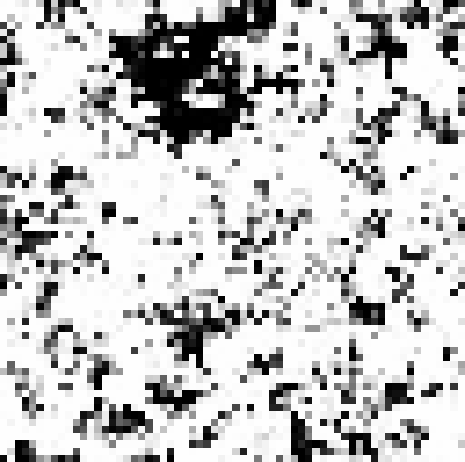
\includegraphics[width=0.6\textwidth]{imgs/broken.png}
        \caption{broken phase \\($m_0^2=-1.0$)}
      \end{subfigure}%
      \hfill
      \begin{subfigure}[b]{0.3\textwidth}\centering
        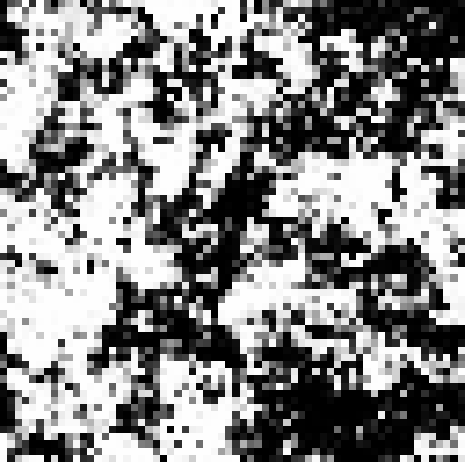
\includegraphics[width=0.6\textwidth]{imgs/transition.png}
        \caption{transition \\($m_0^2=-0.7$)}
      \end{subfigure}%
      \hfill
      \begin{subfigure}[b]{0.3\textwidth}\centering
        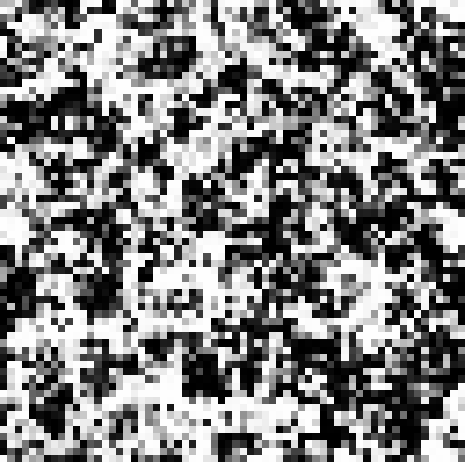
\includegraphics[width=0.6\textwidth]{imgs/symmetric.png}
        \caption{symmetric phase \\($m_0^2=-0.4$)}
      \end{subfigure}
      \hfill
      \caption{\label{fig:primary observables} Visualization of broken phase, symmetric phase and transition. Simulation run on $64\times64$ lattice, plotted after 1000 sweep thermalization.}
  \end{center}
\end{figure}

\begin{table}[h]
    \begin{center}
    {\renewcommand{\arraystretch}{1.2} %
    \begin{tabular}{ c|| c | c | c}
        & broken & transition & symmetric \\ \hline
        $|\bar\phi|$ & 0.56 & 0.07 & 0.02 \\ 
        $S_E/L^2$ & 0.29 & 0.40 & 0.44
    \end{tabular}}

    \end{center}
    \caption{\label{tab:primary observables} Average magnetization with average action per site corresponding to the particular configurations in Fig.~\ref{fig:primary observables}.}
\end{table}

\subsubsection{Average Magnetization}
\label{sec:avg mag}
The average magnetization quantifies the total alignment of the field. In both theories, a value of zero indicates the symmetric phase while a nonzero value indicates broken symmetry. In the NLSM, a magnitude of one represents total alignment.

Due to the $\phi\rightarrow-\phi$ symmetry of the $\phi^4$ model, the ensemble mean of the average magnetization $\langle \phi \rangle$ is $0$. Likewise, the $O(3)$ symmetry in the NLSM enforces $\langle \e \rangle$. To measure the alignment, we therefore use the magnitude of this quantity, defined in the $\phi^4$ model as 
\begin{equation}
|\bar\phi| \equiv \frac{1}{L^2}\left| \sum_i^{L^2} \phi(x_i)\right|.
\end{equation}
and in the NLSM as
\begin{equation}
    |\bar\e| \equiv \frac{1}{L^2}\left|\sum_i^{L^2} \e(x_i)\right|.
\end{equation}

In the symmetric phase, both $\langle \bar\e \rangle$ and $\langle \bar\phi \rangle = 0$ while in the broken phase they are both nonzero.

\subsubsection{Magnetic Susceptibility}
Despite being the prototypical indicator of a phase transition, the magnitude of the magnetization is not always clear on a discretized lattice. For this reason, we consider other observables such as the magnetic susceptibility. Generally, this value is defined as 
\begin{equation}
    \chi_m \equiv L^2 \big(\langle {\bar e}^2 \rangle - \langle \bar e \rangle^2\big)
\end{equation}
in the NLSM (the $\phi^2$ expression is nearly identical). Manifestly, this expression appears as a secondary observable since it is not defined for each lattice configuration. However, due to the rotation invariance of both fields, the second term disappears (see Sec.~\ref{sec:avg mag}), yielding
\begin{align}
    \chi_m &= L^2 \left\langle \left( \sum_x e(x) \right)^2\right\rangle  \\
           &= L^2 \left\langle \sum_{x,y}\e(x)\cdot \e(y) \right\rangle. 
\end{align}
Due to translational invariance from the periodic boundary conditions, this expression becomes
\begin{equation}
    \chi_m = \left\langle \sum_x \e(0)\cdot\e(x) \right\rangle
\end{equation}
for the NLSM. Following the same logic, we derive 
\begin{equation}
    \chi_m = \left\langle \sum_x \phi(0)\phi(x) \right\rangle
\end{equation}
for the $\phi^4$ model.

\subsubsection{Internal Energy}
The internal energy is defined as \cite{berg1981}
\begin{equation}
    E = \frac{2}{\beta L^2} \langle S \rangle
\end{equation}
in the NLSM.


\subsection{Secondary Observables}
Unlike primary observables, secondary observables are defined for each \textit{ensemble}, not each configuration. To further ensure an accurate perspective of the phase transition in the $\phi^4$ model, we incorporate two indicators: the Binder cumulant and the bimodality. Since we do not measure these observables on the NLSM, we do not include their analogous expressions here.

\subsubsection{Binder Cumulant}
We define the Binder cumulant $U$ as \cite{landau2000}
\begin{equation}
    U \equiv 1-\frac{\langle \bar{\phi^4} \rangle}{3\langle \bar{\phi^2}\rangle^2}.
\end{equation}
Similar to the magnitude of the average magnetization, this formula yields $0$ in the symmetric phase and a nonzero value in the broken phase. This nonzero value i $2/3$ for the Binder cumulant. The advantage of this metric is a sharper transition at the critical $m_0^2$.

\subsection{Bimodality}
The final phase transition indicator we use is the bimodality. In the symmetric phase, the average magnetization $\bar\phi$ centers around $0$ while in the broken phase, these values cluster around two peaks. Qualitatively, this metric measures the separation of these peaks.

We begin by measuring $\bar\phi$ for each configuration. We separate each value into an odd number number of bins, ensuring that there is a bin centered at $\bar\phi=0$. We then calculate the number of configurations $n_0$ in the center bin and the number of configurations $n_{max}$ in the fullest bin. The bimodality is then calculated as
\begin{equation}
    B = 1 - \frac{n_0}{n_{max}}.
\end{equation}
When the configurations are centered around $\bar\phi=0$, i.e. the symmetric phase, this value is $0$. When the configurations are aligned such that $\bar\phi\neq0$, i.e. the broken phase, this value becomes $1$.
\subsection{Jackknife Method}
Though it simple to measure the uncertainties associated with primary observables, secondary observables make this process more complicated. While we could propagate the uncertainty of the Binder cumulant, such a process is not clear for the bimodality. Therefore, we utilize a method known Jackknife resampling. 

We begin by calculating some observable $O$ on an ensemble of $N$ configurations. Then, for each configuration $i$, we calculate the same observable but exclude said configuration. This leaves us with a set of $N$ observables $O_i$. Assuming independent measurements, we can calculate the variance of $O$ as
\begin{equation}
    \mathrm{Var}(O) = \sum_{i} \left(C_i - C\right)^2.
\end{equation}
We use this formula to calculate all uncertainties in this study.
\section{Topological Observables}
\label{sec:topological charge}
The $O(3)$ non-linear sigma model model features topological properties originating from two properties: 
\begin{enumerate}
    \item At $x\rightarrow\infty$, the field must become uniform since the Lagrangian must vanish. This allows us to model $x\rightarrow\infty$ as a single point on the field, forming a Riemann sphere in three dimensions.
    \item The elements of the $O(3)$ non-linear sigma model are three-dimensional unit vectors, thereby existing on a three dimensional unit sphere. 
\end{enumerate}

With these two properties, we can view the field as a continuous mapping between two 3D spheres, denoted as $S^2$, and associate an integer number of wrappings to each mapping from $S^2$ to $S^2$. We can envision a tangible metaphor for this wrapping with a balloon and a baseball: by simply inserting the baseball into the balloon, we have established a mapping from every point on the balloon to every point on the baseball. We can create an equally valid map by twisting the balloon's mouth and wrapping the baseball again. In a purely mathematical world, we perform this process an infinite number of times, thereby associating every possible mapping with an integer. The group of integers is known as the \textit{homotopy group} of the non-linear sigma model. We associate every field configuration with an element of this group, known as the \textit{topological charge}, which we denote as $Q$.

In practice, this quantity is nontrivial to calculate. To begin, we define a local topological charge density $q$, defined for each square of adjacent lattice points. This square, known as a \textit{plaquette}, is denoted $x^*$. The global charge $Q$ is the sum of all local charges:
\begin{equation}
    Q \equiv \sum_{x^*} q(x^*).
\end{equation}
As a function of $x^*$, the charge density is a function of the field on the plaquette vertices, an idea visualized in Fig.~\ref{fig:plaquette}.
\begin{figure}
    \centering
    \begin{tikzpicture}
        \draw[step=4cm,gray,thin] (-2,-2) grid (6,6);
        \draw[dotted] (0,0) -- (4,4);
        \draw[thick](0,0) node[circle,fill,inner sep=0pt, minimum size=0.3cm]{} node[anchor=north west] {$x_1$} -- 
                    (0,4) node[circle,fill,inner sep=0pt, minimum size=0.3cm]{} node[anchor=north west] {$x_2$} -- 
                    (4,4) node[circle,fill,inner sep=0pt, minimum size=0.3cm]{} node[anchor=north west] {$x_3$} -- 
                    (4,0) node[circle,fill,inner sep=0pt, minimum size=0.3cm]{} node[anchor=north west] {$x_4$} -- cycle ;
                    \draw[] (2,2) node[circle,fill,inner sep=0pt, minimum size=0.3cm]{} node[anchor=north east]{$x^*$};


        \draw[-stealth] (0.2,1) -- (0.2,3);
        \draw[-stealth] (1,3.8) -- (3,3.8);
        \draw[-stealth] (3,3.5) -- (1,1.5);

        \draw[-stealth] (1,0.5) -- (3,2.5);
        \draw[-stealth] (3.8,3) -- (3.8,1);
        \draw[-stealth] (3,0.2) -- (1,0.2);
    \end{tikzpicture}
    \caption{\label{fig:plaquette} Visualization of plaquette $x^*$. Dotted line separated plaquette into two signed areas which are used to define the topological charge density $q(x^*)$. Arrows represent order of signed area.}
\end{figure}
In the NLSM, the field at each of these vertices is a point on the sphere $S^2$. Therefore, there is a signed area $A$ on the sphere associated with each triplet of points, as shown in Fig.~\ref{fig:sphere} (the sign changes with odd permutations of the ordering). We follow the derivation in \cite{berg1981} and split the plaquette into two triangles, as shown in Fig.~\ref{fig:plaquette}, with the ordering determining the sign. The topological charge density is defined using this signed area as
\begin{equation}
    q(x^*) = \frac{1}{4\pi} \bigg[A\Big(\e(x_1), \e(x_3), \e(x_3)\Big) + A\Big(\e(x_1), \e(x_3), \e(x_4)\Big) \bigg].
\end{equation}
This sign is defined if $A\neq 0, 2\pi$, or in other words, as long as the three points on the sphere are distinct and do not form a hemisphere. In numerical calculations, these points can be ignored. Therefore, we impose that the signed area is defined on the smallest spherical triangle, or mathematically
\begin{equation}
    -2\pi < A < 2\pi.
\end{equation}


Following \cite{berg1981}, this yields an expression for the signed area
\begin{equation}
    A(\e_1, \e_2, \e_1) = 2 \:\mathrm{arg}\Big(1+\e_1\cdot\e_2 + \e_2\cdot\e_3 + \e_3\cdot\e_1 + i\e_1 \cdot (\e_2\times\e_3)\Big).
\end{equation}
Under periodic boundary conditions, these triangles on the sphere necessarily wrap $S^2$ an integer number of times, ensuring $Q$ is an integer.
\begin{figure}[h]
\centering
\begin{tikzpicture}
    \pgfdeclarelayer{nodelayer}
    \pgfdeclarelayer{edgelayer}
    \pgfdeclareradialshading{sphere4}{\pgfpoint{-0.2cm}{0.5cm}}% 
        {rgb(0cm)=(1,1,1);
        rgb(1cm)=(0.5,0.5,0.5); rgb(1.05cm)=(1,1,1)}
        %rgb(0.7cm)=(0.1,0.1,0.1); rgb(1cm)=(0.5,0.05,0); rgb(1.05cm)=(1,1,1)}
    \pgfsetlayers{nodelayer,edgelayer}
    \tikzstyle{label}=[fill=none, draw=none, shape=circle]
    \tikzstyle{point}=[inner sep=0pt, minimum size=0.2cm,fill=black, draw, shape=circle]
    %\tikzstyle{interior line}=[{Stealth[scale=1.5]}-,dotted,thick]
    \tikzstyle{interior line}=[dotted,thick]

    \tikzstyle{triangle}=[thick]
    \tikzstyle{arrow}=[->, thick]
	\begin{pgfonlayer}{nodelayer}
		\node [style=point] (4) at (0.5, 2.5) {};
		\node [style=point] (5) at (0.55, 0.625) {};
		\node [style=point] (6) at (2.25, 0.75) {};
		\node (7) at (0, 0) {};
		\node (8) at (1.25, 1.375) {};
		\node (9) at (2.425, 2.525) {};
	\end{pgfonlayer}
	\begin{pgfonlayer}{edgelayer}
        \draw (0,0) circle (3cm);
        %\shade[inner color=white,outer color=lightgray] (0,0) circle (3cm);
        \shade[shading=sphere4] (0,0) circle (3cm);
		\draw [bend left=15,style=triangle] (4.center) to (6.center);
		\draw [bend left=355,style=triangle] (6.center) to (5.center);
		\draw [bend right=5,style=triangle] (5.center) to (4.center);
		\draw [style=interior line] (4.center) to (7.center);
		\draw [style=interior line] (5.center) to (7.center);
        \draw [style=interior line] (6.center) to (7.center);
        \draw [fill=gray!80] (4.center) to [bend left=15] (6.center) to [bend left=355] (5.center) to [bend right=5] cycle;

		%\draw [style=arrow] (8.center) to (9.center);

        \node [style=label, anchor=north] at (2.25, 0.75) {\small $\e(x_1)$};
        \node [style=label, anchor=north] at (0.55, 0.625) {\small $\e(x_2)$};
        \node [style=label, anchor=east] at (0.5, 2.5) {\small $\e(x_3)$};
		\node [style=point] at (4){};
		\node [style=point] at (5){};
		\node [style=point] at (6){};

        \node [style=label] at (8) {\small $A$};
	\end{pgfonlayer}
\end{tikzpicture}
\caption{\label{fig:sphere} Visualization of signed area $A$ on the sphere $S^2$ traced out by field at points $x_1$, $x_2$ and $x_3$.}
\end{figure}

Following this quantity, we can define a topological susceptibility $\chi_t$
\begin{equation}
\chi_t \equiv \frac{1}{L^2} \Big( \langle Q^2 \rangle - \langle Q \rangle^2 \Big).
\end{equation}
In the trivial case, $\langle Q \rangle$ disappears and   
\begin{equation}
    \chi_t = \frac{1}{L^2} \sum_{x,y} \langle q(x)q(y)\rangle.
\end{equation}
Assuming periodic boundary conditions and therefore translational symmetry, this expression simplifies to 
\begin{equation}
    \chi_t = \frac{1}{L^2} \sum_{x} \langle q(x)q(0)\rangle.
\end{equation}

On the lattice, this quantity is known to diverge in the continuum limit.\cite{bietenholz2018}

\subsection{NLSM $\theta$ term}

In the nonlinear sigma model, we expect $\langle Q \rangle=0$. By introducing a $\theta$ term into the action,
\begin{equation}
    S[\e] \rightarrow S[\e] - i \theta Q[\phi],
\end{equation}
we can construct a topologically nontrivial model (that is, $\langle Q \rangle \neq 0$).

\section{Ultraviolet Divergences}

In Section~\ref{sec:pathintegral},  we defined a fundamental equation of quantum fields using a ``path integral'' which encompasses an uncountably infinite configuration space. However, we said nothing of the integral's convergence. In fact, many fundamental processes in QFT have divergent amplitudes, yielding nonsensical results. The most type of divergence stems from high-momentum states, giving them the name ``ultraviolet divergences''. The remedy to this catastrophe is unintuitive. Essentially, we adopt infinite values for the parameters of the Lagrangian ($m_0^2$ and $\lambda$ in $\phi^4$ theory). Since neither of these two quantities is ever measured directly, we do not have to assume that their values are finite. In practice, this technique is involved and consists of two steps: regularization and renormalization.

\subsection{Regularization: fields on the lattice}
Regularization is a process which introduces a new parameter into calculations. One example is a momentum cutoff. This technique transforms infinite momentum integrals as follows:  
\begin{equation*}
    \int_0^\infty dk \rightarrow \int_0^\Lambda dk,
\end{equation*}
introducing $\Lambda$ as a regularization parameter. This process makes results $\Lambda$-dependent, but finite. Another example is dimensional regularization, which calculates results in terms of the spacetime dimension $d$ and analytically continues this parameter into the real numbers. 

In this study, we employ lattice regularization. This process discretizes the field, modeling the field $\phi(x)$ as a lattice $\phi_i$ where $i$ indexes lattice sites. The inherent parameter in this case is the lattice spacing $a$ which measures the width of each lattice chunk.

\subsection{Renormalization}
After regularization, we redefine the Lagrangian parameters in terms of the regularization parameter, following a handful of boundary conditions. In this study, we assert that $L/\xi$ remains constant, where $L$ is the side length of the system and $\xi$ is the coherence length. In perturbation theory, this process is arduous and includes the introduction of counter-terms into the Lagrangian. In the case of the non-linear sigma model, it is impossible using counterterms\citeneeded but can be performed numerically. In this study, we use predetermined values from \cite{bietenholz2018}.

At this point, we can calculate observables as functions of regularization parameters. To achieve physical values, we take the limit as the regularization parameters approach their physical values. With a momentum cutoff, we take $\Lambda \rightarrow \infty$ and with dimensional regularization we usually take $d\rightarrow 4$. With lattice regularization, we approach the continuum, taking the lattice spacing $a\rightarrow 0$. 

At this point, we have surely eliminated all divergences, right? Unfortunately, this is not always the case. The topological susceptibility $\chi_t$ is one such value that diverges in the continuum limit. As we decrease the width of each lattice site, high frequency modes become more significant, leading to an ultraviolet divergence in the operator. 

\subsection{The Gradient Flow}
\label{sec:gradflow}
To remove this ultraviolet divergence, we adopt a technique is ``smearing'', a local averaging of the field.\cite{solbrig2007} Specifically, we use a technique known as the ``gradient flow'' \cite{monahan2015} which introduces a new half-dimension called ``flow time'', or $\tau$.\footnote{The term ``half-dimension'' indicates that $\tau>0$.}  The flow time parameterizes the smearing such that an evolution in flow time corresponds to suppressing ultraviolet divergences. 

Specifically, the gradient flow pushes field configuration toward classical minima of the action. Additionally, renormalized correlation functions remain renormalized at nonzero flow time.\cite{luscher2013} In 2D $\phi^4$ scalar field theory, the gradient flow is defined by the differential equation 
\begin{equation}
    \frac{\partial \rho(\tau, x)}{\partial \tau} = \partial^2 \rho(\tau,x)
\end{equation}
where $\partial^2$ is the Laplacian in 4-D Euclidean spacetime and $\tau$ is the flow time. Here, $\rho$ is the field evolved into a nonzero flow time, bounded by the condition $\rho(\tau=0,x) = \phi(x)$. In the $\phi^4$ theory, we can solve this equation exactly to find \cite{monahan2016}
\begin{equation}
    \rho(\tau, x) = \frac{1}{4 \pi \tau} \int d^2 y e^{-(x-y)^2/4\tau} \phi(y).
\end{equation}
This function forms a Gaussian, smoothly dampening high-momentum modes and removing ultraviolet divergences from evolved correlation functions.\cite{makino2015a} We can visualize this by plotting the $\phi$ field, shown in Fig.~\ref{fig:flow}. These plots demonstrate the reduction of high momentum modes.

\begin{figure}[h]
  \centering
      \begin{subfigure}[b]{0.2\textwidth}\centering
        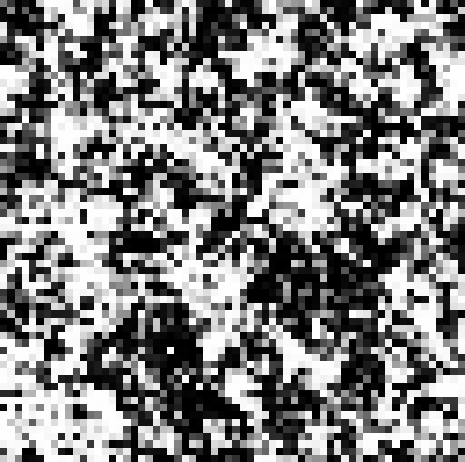
\includegraphics[width=0.9\textwidth]{imgs/gf0.png}
        \caption{$\tau=0$}
      \end{subfigure}%
      \begin{subfigure}[b]{0.2\textwidth}\centering
        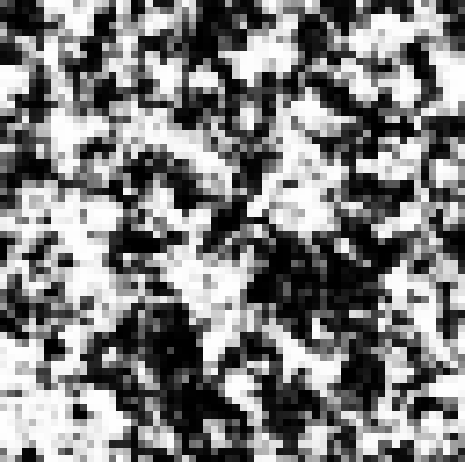
\includegraphics[width=0.9\textwidth]{imgs/gf1.png}
        \caption{$\tau=0.001$}
      \end{subfigure}%
      \begin{subfigure}[b]{0.2\textwidth}\centering
        
\includegraphics[width=0.9\textwidth]{imgs/gf2.png}
        \caption{$\tau=0.01$}
      \end{subfigure}%
      \begin{subfigure}[b]{0.2\textwidth}\centering
        
\includegraphics[width=0.9\textwidth]{imgs/gf3.png}
        \caption{$\tau=0.1$}
      \end{subfigure}%
      \caption{\label{fig:flow} Effect of flow time evolution on a random lattice in the symmetric phase. White represents positive values of $\phi$ while black represents negative.}
\end{figure}

Generally, we can choose any flow time equation that drives the field towards a classical minimum. Beyond the $\phi^4$ model, we need flow equations that incorporate different types of fields. In the non-linear sigma model, it has been shown that an appropriate manifestation of the flow time can resolve divergences \cite{makino2015a}. Therefore, it is possible to define a different flow equation for this model as well. Following \cite{bietenholz2018}, we can define the gradient flow in this model via the differential equation
\begin{equation}
    \label{eq:nsm_gradflow}
    \partial_\tau \vec\rho (\tau,x) = \left( 1 - \vec\rho(\tau,x) \vec\rho(\tau,x)^T \right) \partial^2 \vec\rho(\tau,x),
\end{equation}
where $\partial^2$ is the Laplacian operator in Euclidean space\footnote{Explicitly, $\partial^2 = \frac{\partial^2}{\partial t^2} + \nabla^2$}. We solve this equation numerically using the boundary condition $\vec\rho(0,x) = \e(x)$.



\chapter{Methods}
\label{sec:methods}
Our study of the gradient flow in the non-linear sigma model consists of a computational part and an analytical part. We begin by outlining a numerical Monte Carlo method to simulate the lattice in two and three dimensions. We verify our program with the well-studied $\phi^4$ scalar field theory. We then generalize our model to a vector field to simulate the non-linear sigma model. This simulation system provides data on vacuum states with which we study the gradient flow's effect on topology.

We implement these two algorithms first in Python for the $\phi^4$ model. Afterwards, we transition to C/C++ code due to the increased speed for more complicated theories. 
\section{Fields on the Lattice}
To implement the lattice regularization technique, we must redefine the field action in terms of discrete positions, a process known as ``discretization''. We transition from $x$ as a continuous vector in $\mathbb{R}^2$ to $x_{i,j}$ where
\begin{equation}
    x_{i,j} = ia \hat{\mu}_t + j a \hat{\mu}_x.
\end{equation}
Here, $a$ is the lattice constant and $\hat{\mu}_0$ and $\hat{\mu}_1$ are unit vectors. This change effectively shifts the domain of the field from $\mathbb{R}^2$, which is uncountably infinite, to $\mathbb{Z}^2$, which is countably infinite. To achieve a finite domain, we impose periodic boundary conditions, such that 
\begin{equation}
    \phi\left(x_{i+L,j}\right) = \phi\left(x_{i,j+L}\right) = \phi\left(x_{i,j}\right)
\end{equation}
where $L$ is the side length (in units of the lattice constant $a$) of the system. In this study we focus solely on square geometries and thus the side length $L$ is unambiguous.

In the $\phi^4$ model, we can specify a discrete action using the Euclidean action from Eq. \ref{eq:phi4 euclidean action}. We begin by redefining the derivative operator as a difference:
\begin{align}
    \partial_\mu \phi = \frac{\phi\left(x + a \hat{\mu}\right) - \phi(x)}{a}
\end{align}
We can then define the kinetic term
\begin{align}
    \half \left(\partial_t\phi\right)^2 + \half \left(\partial_x\phi\right)^2 \rightarrow& \frac{1}{2a^2}\left[ \left(\phi(x+a \hat{t}) -\phi(x)\right)^2 + \left(\phi(x+a \hat{x}) -\phi(x)\right)^2\right] \\
    \begin{split} \rightarrow& \frac{1}{2a^2}\left[ \phi^2(x+a\hat{t}) + \phi^2(x+a\hat{x}) + 2\phi^2(x)\right.\\ &\qquad \left.- 2\phi(x+a\hat{t})\phi(x) - 2\phi(x+a\hat{x})\phi(x) \right]\hfilneg\end{split}
\end{align}
Since we will eventually sum over all sites $x$, the periodic boundary conditions imply that an overall shift in $x$ does not effect the final action. Therefore, we can combine the first two terms with the third term to produce 
\begin{equation}
    \half \left(\partial_t\phi\right)^2 + \half \left(\partial_x\phi\right)^2 \rightarrow \frac{1}{a^2}\left[ 2\phi^2(x) - \phi(x+a\hat{t})\phi(x) - \phi(x+a\hat{x})\phi(x) \right]
\end{equation}
Unlike the kinetic term, the mass and interaction terms remain unchanged under the discretization procedure. The only remaining change is a shift from an integral to a sum. This takes the form
\begin{equation}
    \int dtdx \rightarrow a^2 \sum_i
\end{equation}
such that the final discretized action becomes
\begin{equation}
    \label{eq:phi4 discretized action}
    S_{\mathrm{lat}}[\phi] = \sum_i \left[-\phi(x_i + a\hat{t})\phi(x_i) - \phi(x_i + a\hat{x})\phi(x_i) + \left(2+\half m_0^2\right)\phi^2(x_i) + \frac{1}{4}\lambda \phi^4(x_i)\right]
\end{equation}

Likewise, we can discretize the non-linear sigma model. In this case, the derivative term becomes 
\begin{equation}
    \half \left(\partial_t\e\right)^2 + \half \left(\partial_x\e\right)^2 \rightarrow \frac{1}{a^2}\left[ 2 - \e(x+a\hat{t})\cdot\e(x) - \e(x+a\hat{x})\cdot\e(x) \right].
\end{equation}
Note that we have used the identity $\e\cdot\e = 1$. Inserting this into Eq.~\ref{eq:nlsm euclidean action} yields the discretized action
\begin{equation}
    \label{eq:nlsm discretized action}
    S_\mathrm{lat}[\e] = \sum_i \left[ 2 - \e(x+a\hat{t})\cdot\e(x) - \e(x+a\hat{x})\cdot\e(x) \right].
\end{equation}

Finally, we redefine the gradient flow in on the lattice. Since the gradient flow is solved exactly in the $\phi^4$ model, we rely on a Fast Fourier Transform. \textit{TODO: explicit expression for this} In the NLSM, the definition of the gradient flow (Eq.~\ref{eq:nsm_gradflow}) becomes 
\begin{equation}
    \label{eq:nsm_gradflow_disc}
    \partial_\tau \e (\tau, x) = \left( 1 - \e(\tau,x) \e(\tau,x)^T\right) \partial^2 \e(\tau,x),
\end{equation}
 where the Laplacian operator $\partial^2$ is defined as
\begin{equation*}
    \partial^2 \e(\tau,x) = \e(\tau, x+a \hat{t}) + \e(\tau,x-a\hat t) + \e(\tau, x+a \hat{x}) + \e(\tau,x-a\hat x) - 2 d \e(t)_x.
\end{equation*}
%TODO: derive the laplacian operator


\section{Monte Carlo Simulations}
\label{sec:mc}
We implement a Markov Chain Monte Carlo method following Schaich's thesis \cite{schaich2006}. This implementation utilizes a ``random walk,'' i.e. a set of random steps through phase space, to determine statistical values such as correlation functions across the lattice. By the definition of the Markov chain, the probability of adoption of each state, and therefore its inclusion in the Monte Carlo calculation, depends only on the current state and the proposed state. This probability is denoted as $P(\mu\rightarrow\nu)$ where $\mu$ and $\nu$ are the existing and proposed lattice configurations respectively.


\subsection{Metropolis Algorithm}
We primarily use the Metropolis algorithm for the calculation of new Markov chain configurations. We begin with a so-called ``hot start,'' where each field value at each lattice site is randomly selected. Then we propose a new value for a single lattice point, which is accepted with a probability
\begin{equation}
    P(\phi_a\rightarrow\phi_b) = \begin{cases} 
        e^{-(S[\phi_b] - S_[\phi_a])} & S[\phi_b] < S_[\phi_a] \\
        1 & \mathrm{otherwise} \\
   \end{cases}
\end{equation}
where $\phi_a$ is the initial configuration and $\phi_b$ is the proposed configuration. This process is performed for each point on the lattice, making up a ``sweep.'' Repeating this sweep many times pushes the lattice toward the action minimum.


\subsection{Wolff Cluster Algorithm}

Though the Metropolis algorithm will slowly find the absolute minimum of the theory, the presence of local minima can greatly prolong the convergence. Both the $\phi^4$ model and the non-linear sigma model feature ``kinetic'' terms with gradients of $\phi$. Therefore, the presence of large similarly-valued regions in the lattice can lead to a local minimum. One method of removing these clusters involves identifying all clusters on the lattice and probabilistically flipping each, a technique known as the Swendsen-Wang algorithm\cite{swendsen1987}. 

A more efficient approach is the Wolff algorithm\cite{wolff1989}, which \textit{grows} one cluster probabilistically and flips it unconditionally. In the case of $\phi^4$ theory, this flipping takes the form of a simple sign change. In the non-linear sigma model we choose a random unit vector $\vec r$ and consider the projection of the field on this vector. When the cluster flips, each site is flipped along this direction.\citeneeded To identify the cluster, the algorithm uses a recursive algorithm defined by the probability of adding a new site, growing the cluster from a single, randomly selected ``seed''. Starting with the seed, the probability of adding each neighboring site is given by the source site $x$ and the proposed site $x'$. Wolff defines this probability for arbitrary sigma models as 
\begin{equation}
    \label{eq:phi4 wolff padd}
    P_{add}(\e(x),\e(x')) = \begin{cases} 
        1 - e^{2\beta [\vec{r} \cdot \e(x)][\vec{r} \cdot \e(x')]} & \mathrm{sgn}[\vec{r}\cdot\e(x)]=\mathrm{sgn}[\vec{r}\cdot\e(x')]\\
        0 & \mathrm{otherwise} \\
   \end{cases}
\end{equation}
This expression is designed to preserve the detailed balance equations. We can demonstrate this quality, and motivate an equivalent expression for the $\phi^4$ model, by considering the probability $P(\phi\rightarrow f_C(\phi))$ of flipping some cluster $C$. Generally,
\begin{equation}
    P\big(\phi \rightarrow f_C\left(\phi\right)\big) \propto \prod_{\langle x,x'\rangle \in \partial C}  \Big[1 - P_{add}\big(\e(x),\e(x')\big)\Big]
\end{equation}
where $\partial C$ is the set of pairs of sites on the boundary of $C$. Since $P_{add}=0$ for unaligned sites, these pairs contribute nothing to the value. We can also find the probability $P(f_C(\phi) \rightarrow \phi)$ with the same expression:
\begin{equation}
P\big(f_C(\phi)\rightarrow \phi \big) \propto \prod_{\langle x,x'\rangle \in \partial C}  \Big[1 - P_{add}\big(\e(x),R\;\e(x')\big)\Big],
\end{equation}
where the matrix $R$ which is a reflection matrix along the vector $\vec{r}$.

From the discretized action of the NLSM model (Eq.~\ref{eq:nlsm discretized action}) and the detailed balance equation (Eq.~\ref{eq:detailedbalance2}), we derive
\begin{equation}
    \prod_{\langle x,x'\rangle \in \partial C}  \frac{ 1 - P_{add}\big(\e(x),\e(x')\big)}{ 1 - P_{add}\big(\e(x),R\;\e(x')\big)}  = \mathrm{exp}\left\{\beta\sum_{\langle x,x'\rangle \in \partial C} \e(x)\cdot[R-1]\e(x')\right\}.
\end{equation}
Note that all the pairs within and outside the cluster cancel in the fraction on the left and the difference on the right. Using the definition of the reflection matrix
\begin{equation}
    R\;\e = \e - 2(\e\cdot\vec{r})\e,
\end{equation}
we can simplify the equation to be 
\begin{equation}
    \prod_{\langle x,x'\rangle \in \partial C}  \frac{ 1 - P_{add}\big(\e(x),\e(x')\big)}{ 1 - P_{add}\big(\e(x),R\;\e(x')\big)}  = \prod_{\langle x,x'\rangle \in \partial C}\mathrm{exp}\big\{2\beta[r\cdot\e(x)][r\cdot\e(x')]\big\}.
\end{equation}
By plugging in Eq.~\ref{eq:phi4 wolff padd}, it is clear to see this equation is satisfied.

Using this same reasoning, we can deduce an expression for $P_{add}$ in the $\phi^4$ model. Since this model is one dimensional, the reflection matrix $R$ is equivalent to $-1$. Adapting the NLSM detailed balance equation for the $\phi$ field, we find
\begin{equation}
    \prod_{\langle x,x'\rangle \in \partial C}  \frac{ 1 - P_{add}\big(\phi(x),\phi(x')\big)}{ 1 - P_{add}\big(\phi(x),-\phi(x')\big)}  = \prod_{\langle x,x'\rangle \in \partial C}\mathrm{exp}\{-2 \phi(x)\phi(x')\}.
\end{equation}
This equation is satisfied by the ansatz
\begin{equation}
    \label{eq:nlsm wolff padd}
    P_{add}(\phi(x),\phi(x')) = \begin{cases} 
        1 - e^{-2\phi(x)\phi(x')]} & \mathrm{sgn}[\phi(x)]=\mathrm{sgn}[\phi(x')]\\
        0 & \mathrm{otherwise} \\
   \end{cases}.
\end{equation}
We will use this expression in the computational implementation of this algorithm.

Fig.~\ref{fig:wolff} shows a real demonstration of this process. We can see a large cluster of negative field values becoming positive. Note that periodic boundary conditions apply, so the small island of black at the bottom is actually part of the larger cluster. Furthermore, this visualization demonstrates the probabilistic nature of the Wolff algorithm. Since states are added probabilistically, there are some small holes in the cluster. These will be removed by following Metropolis sweeps.
\begin{figure}[h]
  \centering
      \begin{subfigure}[b]{0.5\textwidth}\centering
        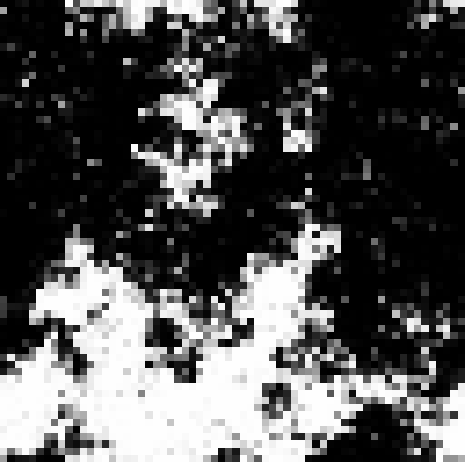
\includegraphics[width=0.6\textwidth]{imgs/wolffa.png}
        \caption{before cluster flip}
      \end{subfigure}%
      \hfill
      \begin{subfigure}[b]{0.5\textwidth}\centering
        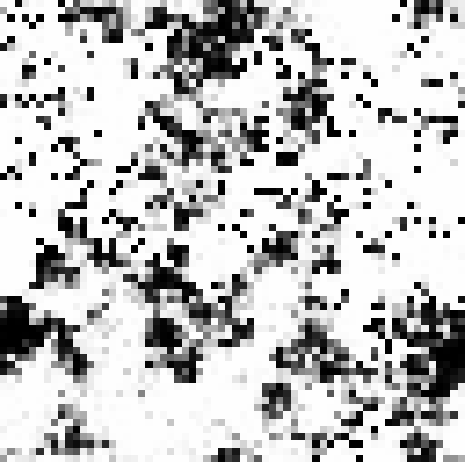
\includegraphics[width=0.6\textwidth]{imgs/wolffb.png}
        \caption{after cluster flip}
      \end{subfigure}
      \hfill
      \caption{\label{fig:wolff} An example of the Wolff cluster algorithm in the $\phi^4$ model. White represents positive values of $\phi$ while black represents negative. $\lambda=0.5$, $m_0^2=-0.9$}
  
\end{figure}

\subsection{Checkerboard algorithm}

In order to parallelize the Metropolis algorithm, we use a checkerboard algorithm. Since the Lagrangian density at each site does not depend on any sites diagonal to it, the lattice can be split into ``white'' sites and ``black'' sites, like the tiles on a checkerboard. Each white site is independent of every other white site and likewise with black sites. Therefore, we can split the sites of each color into separate parallel processing nodes and independently run the Metropolis algorithm, ensuring that no site affects the Lagrangian density at any other site. We use this method to parallelize the code through the Message Passing Interface (MPI).

\subsection{Thermalization}
Since we begin with a random lattice, the first few configurations of our Monte Carlo simulation will be far from the lattice minimum. We plot the action as a function of metropolis sweeps in Fig.~\ref{fig:therm}.
\begin{figure}[h]
  \centering
      \begin{subfigure}[b]{0.5\textwidth}\centering
        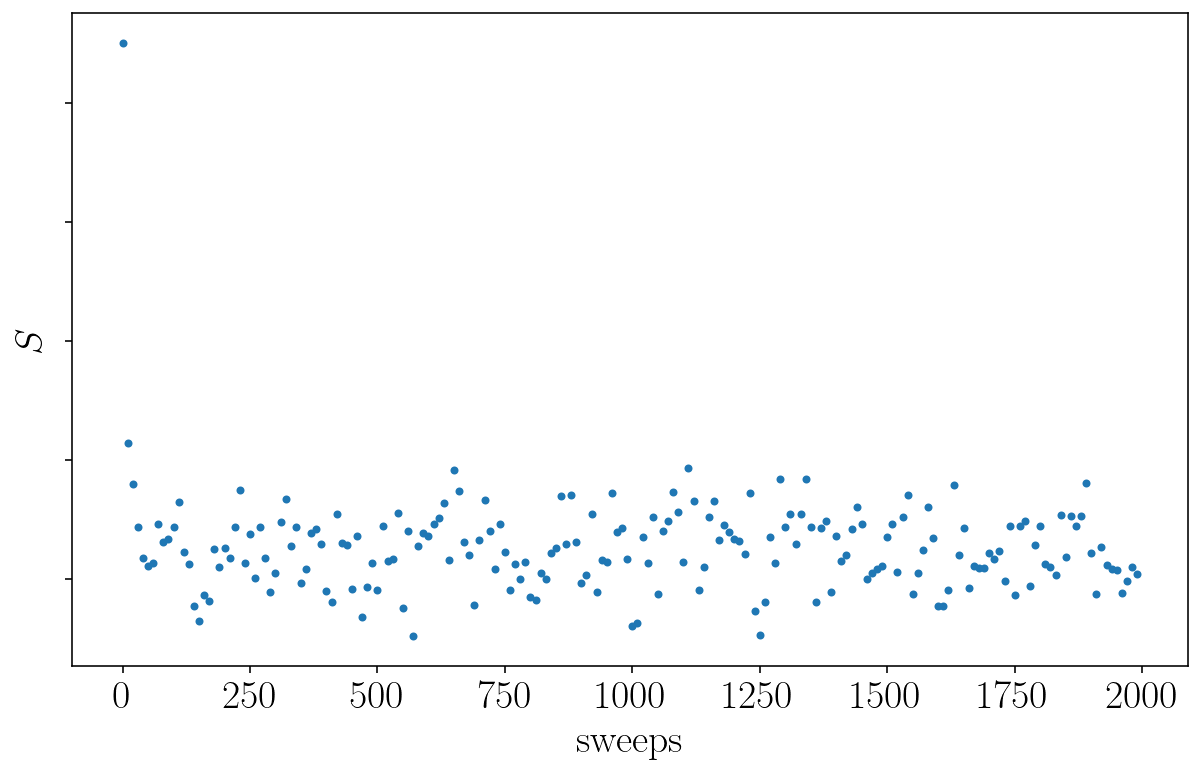
\includegraphics[width=0.6\textwidth]{imgs/therm24.png}
        \caption{$L=24$}
      \end{subfigure}%
      \hfill
      \begin{subfigure}[b]{0.5\textwidth}\centering
        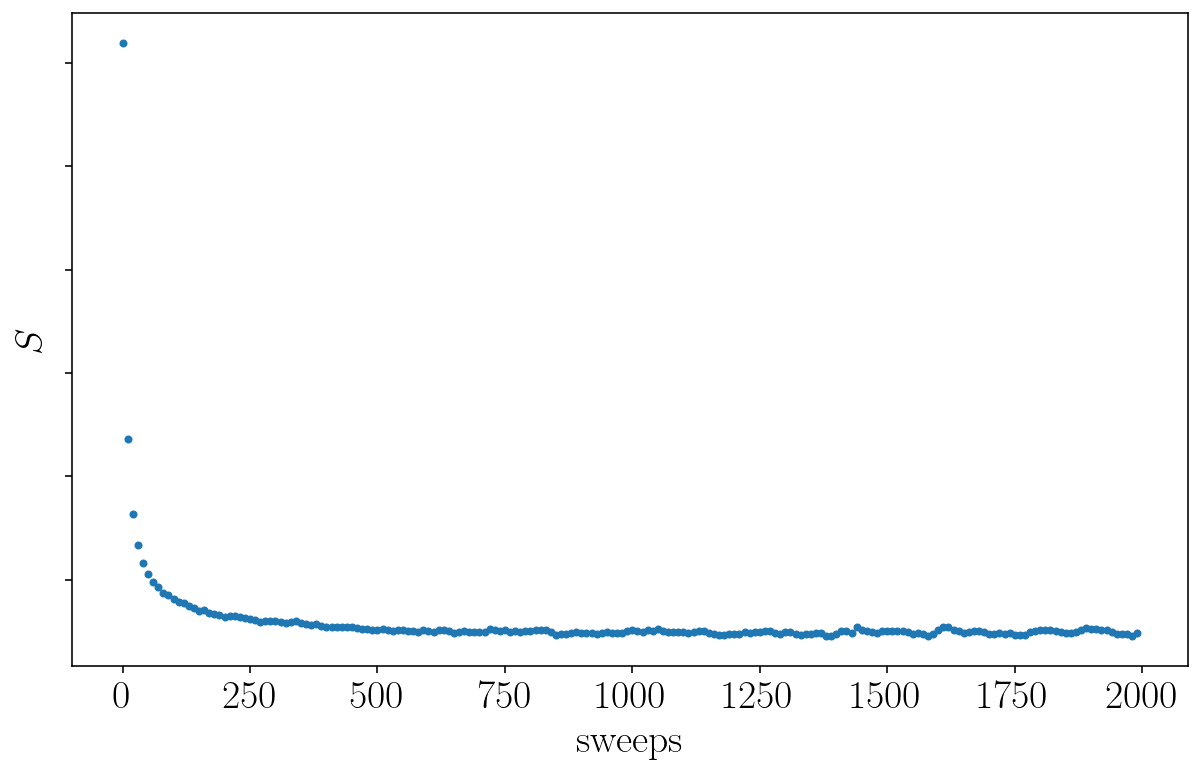
\includegraphics[width=0.6\textwidth]{imgs/therm404.png}
        \caption{$L=404$}
      \end{subfigure}
      \hfill
      \caption{\label{fig:therm} Plots of the action as a function of Monte Carlo time, starting with a random NLSM lattice.}
\end{figure}
Based on this plot, we determine that 1000 sweeps will give sufficient time for the system to reach the classical action minimum. We use this value for the remainder of this study.
\subsection{Autocorrelation times and thermalization}
One important aspect is the correlation between different states of the Markov chain. Ideally, each sample of the lattice would be completely independent, but this is not the case. Since each configuration is based on previous configurations, there is a correlation between each pair of members in the Markov chain, decreasing exponentially based on the number of steps between. Explicitly, the autocorrelation scales as \[e^{t/\tau_{int}}\] where $t$ is the number of steps between configurations and $\tau_{int}$ is the autocorrelation time.\footnote{Though it is called a time, $\tau_{int}$ is in units of Markov Chain steps.} When performing simulations of the lattice, the number of sweeps between measurements should be much larger than $\tau_{int}$. 

    We use Wolff's automatic windowing procedure \cite{wolff2007} and the magnetic susceptibility $\chi_m$ to estimate the autocorrelation. Using Wolff's public MatLab code\footnote{\url{https://www.physik.hu-berlin.de/de/com/ALPHAsoft}}, we estimate the autocorrelation time for $L=24$ and $L=404$ lattices. This algorithm identifies the optimal window size with which to calculate the autocorrelation time. We perform this process on $L=24$ and $L=404$ lattices using a thermalization of $1000$ sweeps and $500$ total measurements. Note that this calculation included a Wolff cluster algorithm every $5$ sweeps. The result of this calculation is shown in Fig.~\ref{fig:tauint}.
\begin{figure}[h]
  \centering
      \begin{subfigure}[b]{0.5\textwidth}\centering
        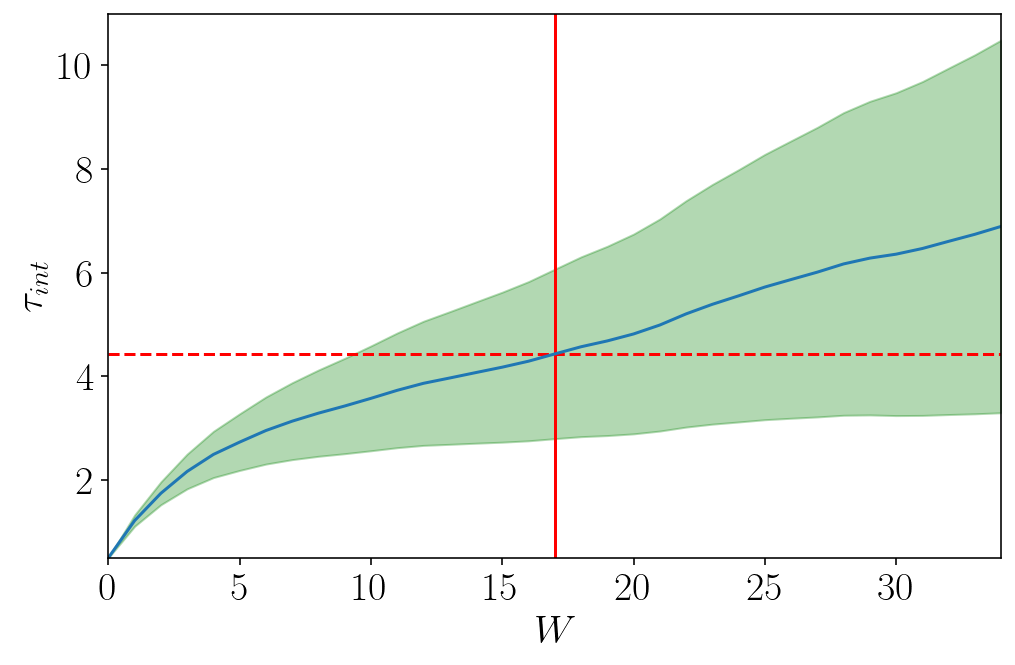
\includegraphics[width=0.6\textwidth]{imgs/tauint24.png}
        \caption{$L=24$, $\tau_{int}=4.43$}
      \end{subfigure}%
      \hfill
      \begin{subfigure}[b]{0.5\textwidth}\centering
        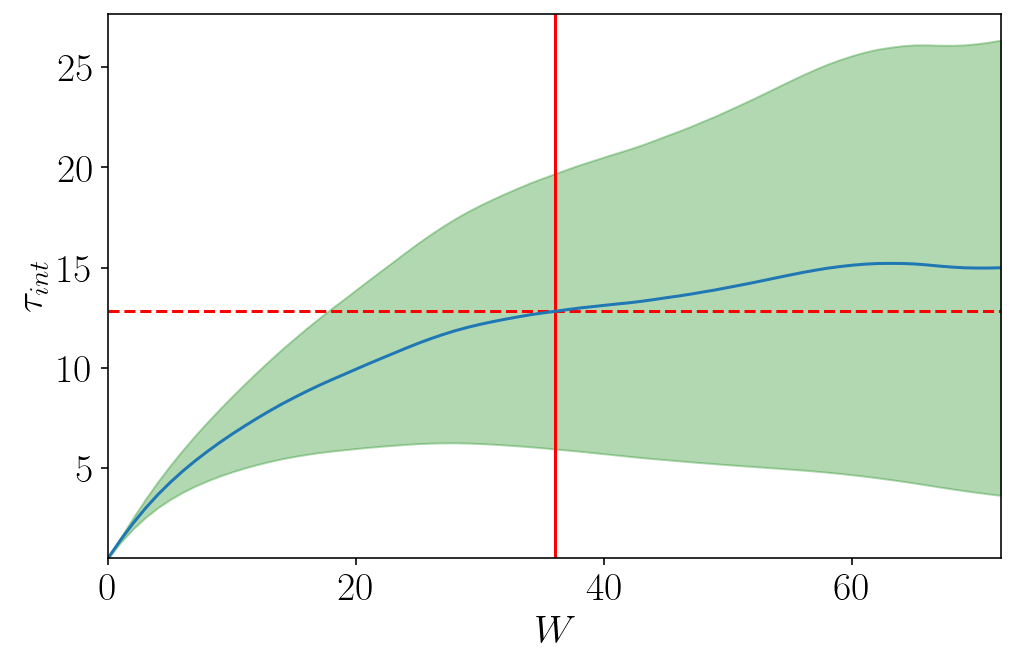
\includegraphics[width=0.6\textwidth]{imgs/tauint404.png}
        \caption{$L=404$, $\tau_{int}=12.81$}
      \end{subfigure}
      \hfill
      \caption{\label{fig:tauint} Plots of automatic windowing procedure used to calculate $\tau_{int}$ for the NLSM model.}
\end{figure}

Based on these two values for $\tau_{int}$, we decide to measure every $50$ sweeps for each simulation. This value will ensure that each measurement is effectively independent.

\subsection{Runge-Kutta Algorithm}
In order to calculate the gradient flow, we numerically solve the differential equation using a fourth-order Runga-Kutta approximation. This algorithm refines the Euler method 
\begin{equation*}
    \e(\tau+h)_x \approx \e(\tau)_x + h f(\e(\tau)_x).
\end{equation*}
where $f(\e)$ is defined for convenience as 
\begin{equation}
    f(\e)=\partial_\tau \e (\tau)_x  = \left( 1 - \e(\tau)_x \e(\tau)_x^T\right) \partial^2 \e(\tau)_x,
\end{equation}
following from Eq.~\ref{eq:nsm_gradflow_disc}. To the fourth order, this approximation becomes 
%
\begin{align}
    \label{eq:rungekutta}
    k_1 &= h f\left(\e\left(\tau\right)_x\right) \\ 
    k_2 &= h f\left(\e\left(\tau\right)_x + \frac{k_1}{2}\right) \\ 
    k_3 &= h f\left(\e\left(\tau\right)_x + \frac{k_2}{2}\right) \\ 
    k_4 &= h f\left(\e\left(\tau\right)_x + k_3\right) \\ 
    \e(\tau+h)_x &= \e(\tau)_x + \frac{k_1}{6} + \frac{k_2}{3} + \frac{k_3}{3} + \frac{k_4}{6} + O(h^5).
\end{align}
This method is usually superior to Euler's method and the midpoint method \cite{vetterling1992}.

To increase the efficiency of this algorithm, we implement the step-doubling algorithm to adaptively adjust $h$. If the error of a Runge-Kutta step is greater than the tolerance, the same step is repeated with half the step size. Alternatively, if the error is less than half of the tolerance, the step size is doubled for the next calculation. Finally, if the step size is greater than the distance to the next measurement, that distance is used as the step size, using the normal value afterwards. Otherwise, the algorithm proceeds with the consistent step size. 


\section{Topological charge with a $\theta$ term}
In Sec.~\ref{sec:topological charge}, we discussed the introduction of a $\theta$ term into the action. This change made the theory ``topological'', pushing $\langle Q \rangle$ away from zero. In order to calculate $\langle Q \rangle$ as a function of $Q$, we consider the path integral
\begin{align}
    \langle Q \rangle_\theta &=\int \mathcal{D}\e\:Q[\e]e^{-S[\e]+i\theta Q[\e]} \\
                             &=\int \mathcal{D}\e\:\left( Q[\e]e^{i\theta Q[\e]} \right) e^{-S[\e]} \\
                             &=\langle Q e^{i \theta Q} \rangle_{\theta=0}.
\end{align}
Therefore, we can calculate $\langle Q \rangle_\theta$ for arbitrary $\theta$ using the same simulation framework as the $\theta=0$ case.

We can also relate this function to the topological susceptibility. By expanding the exponent as a Taylor series around $\theta=0$, we find that  
\begin{equation}
    \langle Q \rangle_\theta = \langle Q \rangle_{\theta=0} + i \theta \langle Q^2 \rangle_{\theta=0} + O(\theta^2),
\end{equation}
such that 
\begin{align}
    -i \frac{\partial}{\partial \theta} \langle Q \rangle_\theta &= \langle Q^2 \rangle_{\theta=0}\\
                                                              &= \chi_t L^2.
\end{align}
We expect to see the slope of this function at zero increase for large lattice sizes.


\chapter{Results}
\section{$\phi^4$ model results}

We initially implemented the $\phi^4$ model using the Monte Carlo method described in Sec.~\ref{sec:methods} to verify the results of our system. According to previous studies (\cite{monahan2016}, \cite{schaich2006}), the $\phi^4$ model exhibits a symmetric and broken phase depending on its parameters $m_0^2$ and $\lambda$, specifically occurring at $m_0^2 = -0.72$ for $\lambda = 0.5$. We verify this result by plotting four observables: the lattice average $|\langle\bar\phi\rangle|$, the lattice variance $\chi$, the Binder cumulant $U$ and the bimodality $B$ in Fig.~\ref{fig:phi4}.
\begin{figure}[h]
    \centering
      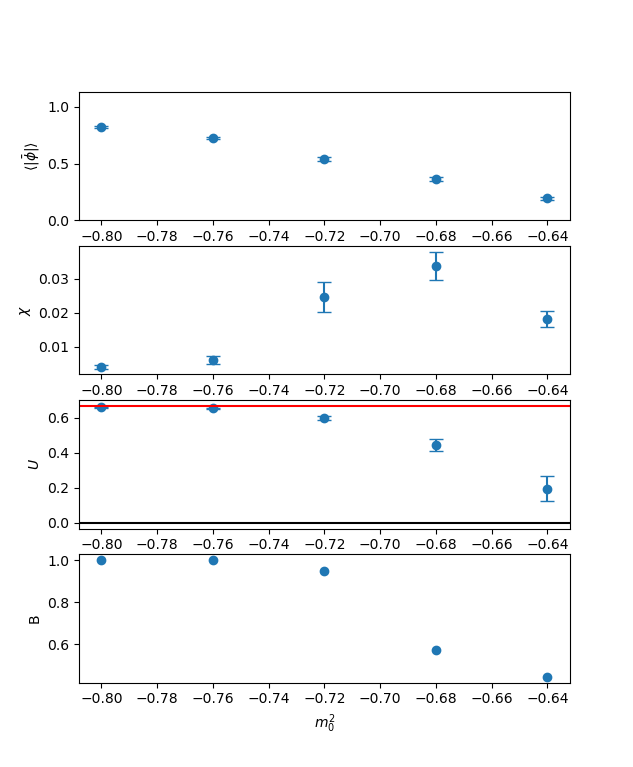
\includegraphics[width=0.7\textwidth]{imgs/phi4.png}
      \caption{\label{fig:phi4} Simulation of the phase transition in the $\phi^4$ model: Magnetization $\langle |\bar\phi|\rangle$, magnetic susceptibility $\chi_m$, Binder cumulant $U$ and bimodality $B$ for various values of the mass squared $m_0^2$.}
\end{figure}

\section{Non-linear sigma model results}
After confirming the phase transition 
\begin{figure}[h]
    \centering
      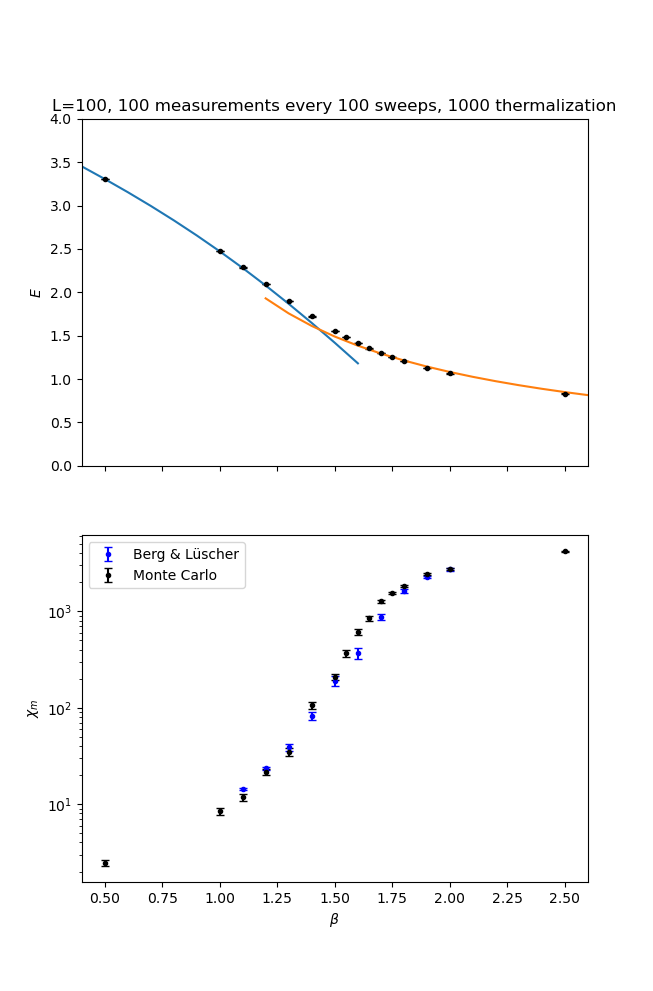
\includegraphics[width=\textwidth]{imgs/internal_energy.png}
      \caption{\label{fig:bergluscher}}
\end{figure}

\begin{figure}[h]
    \centering
      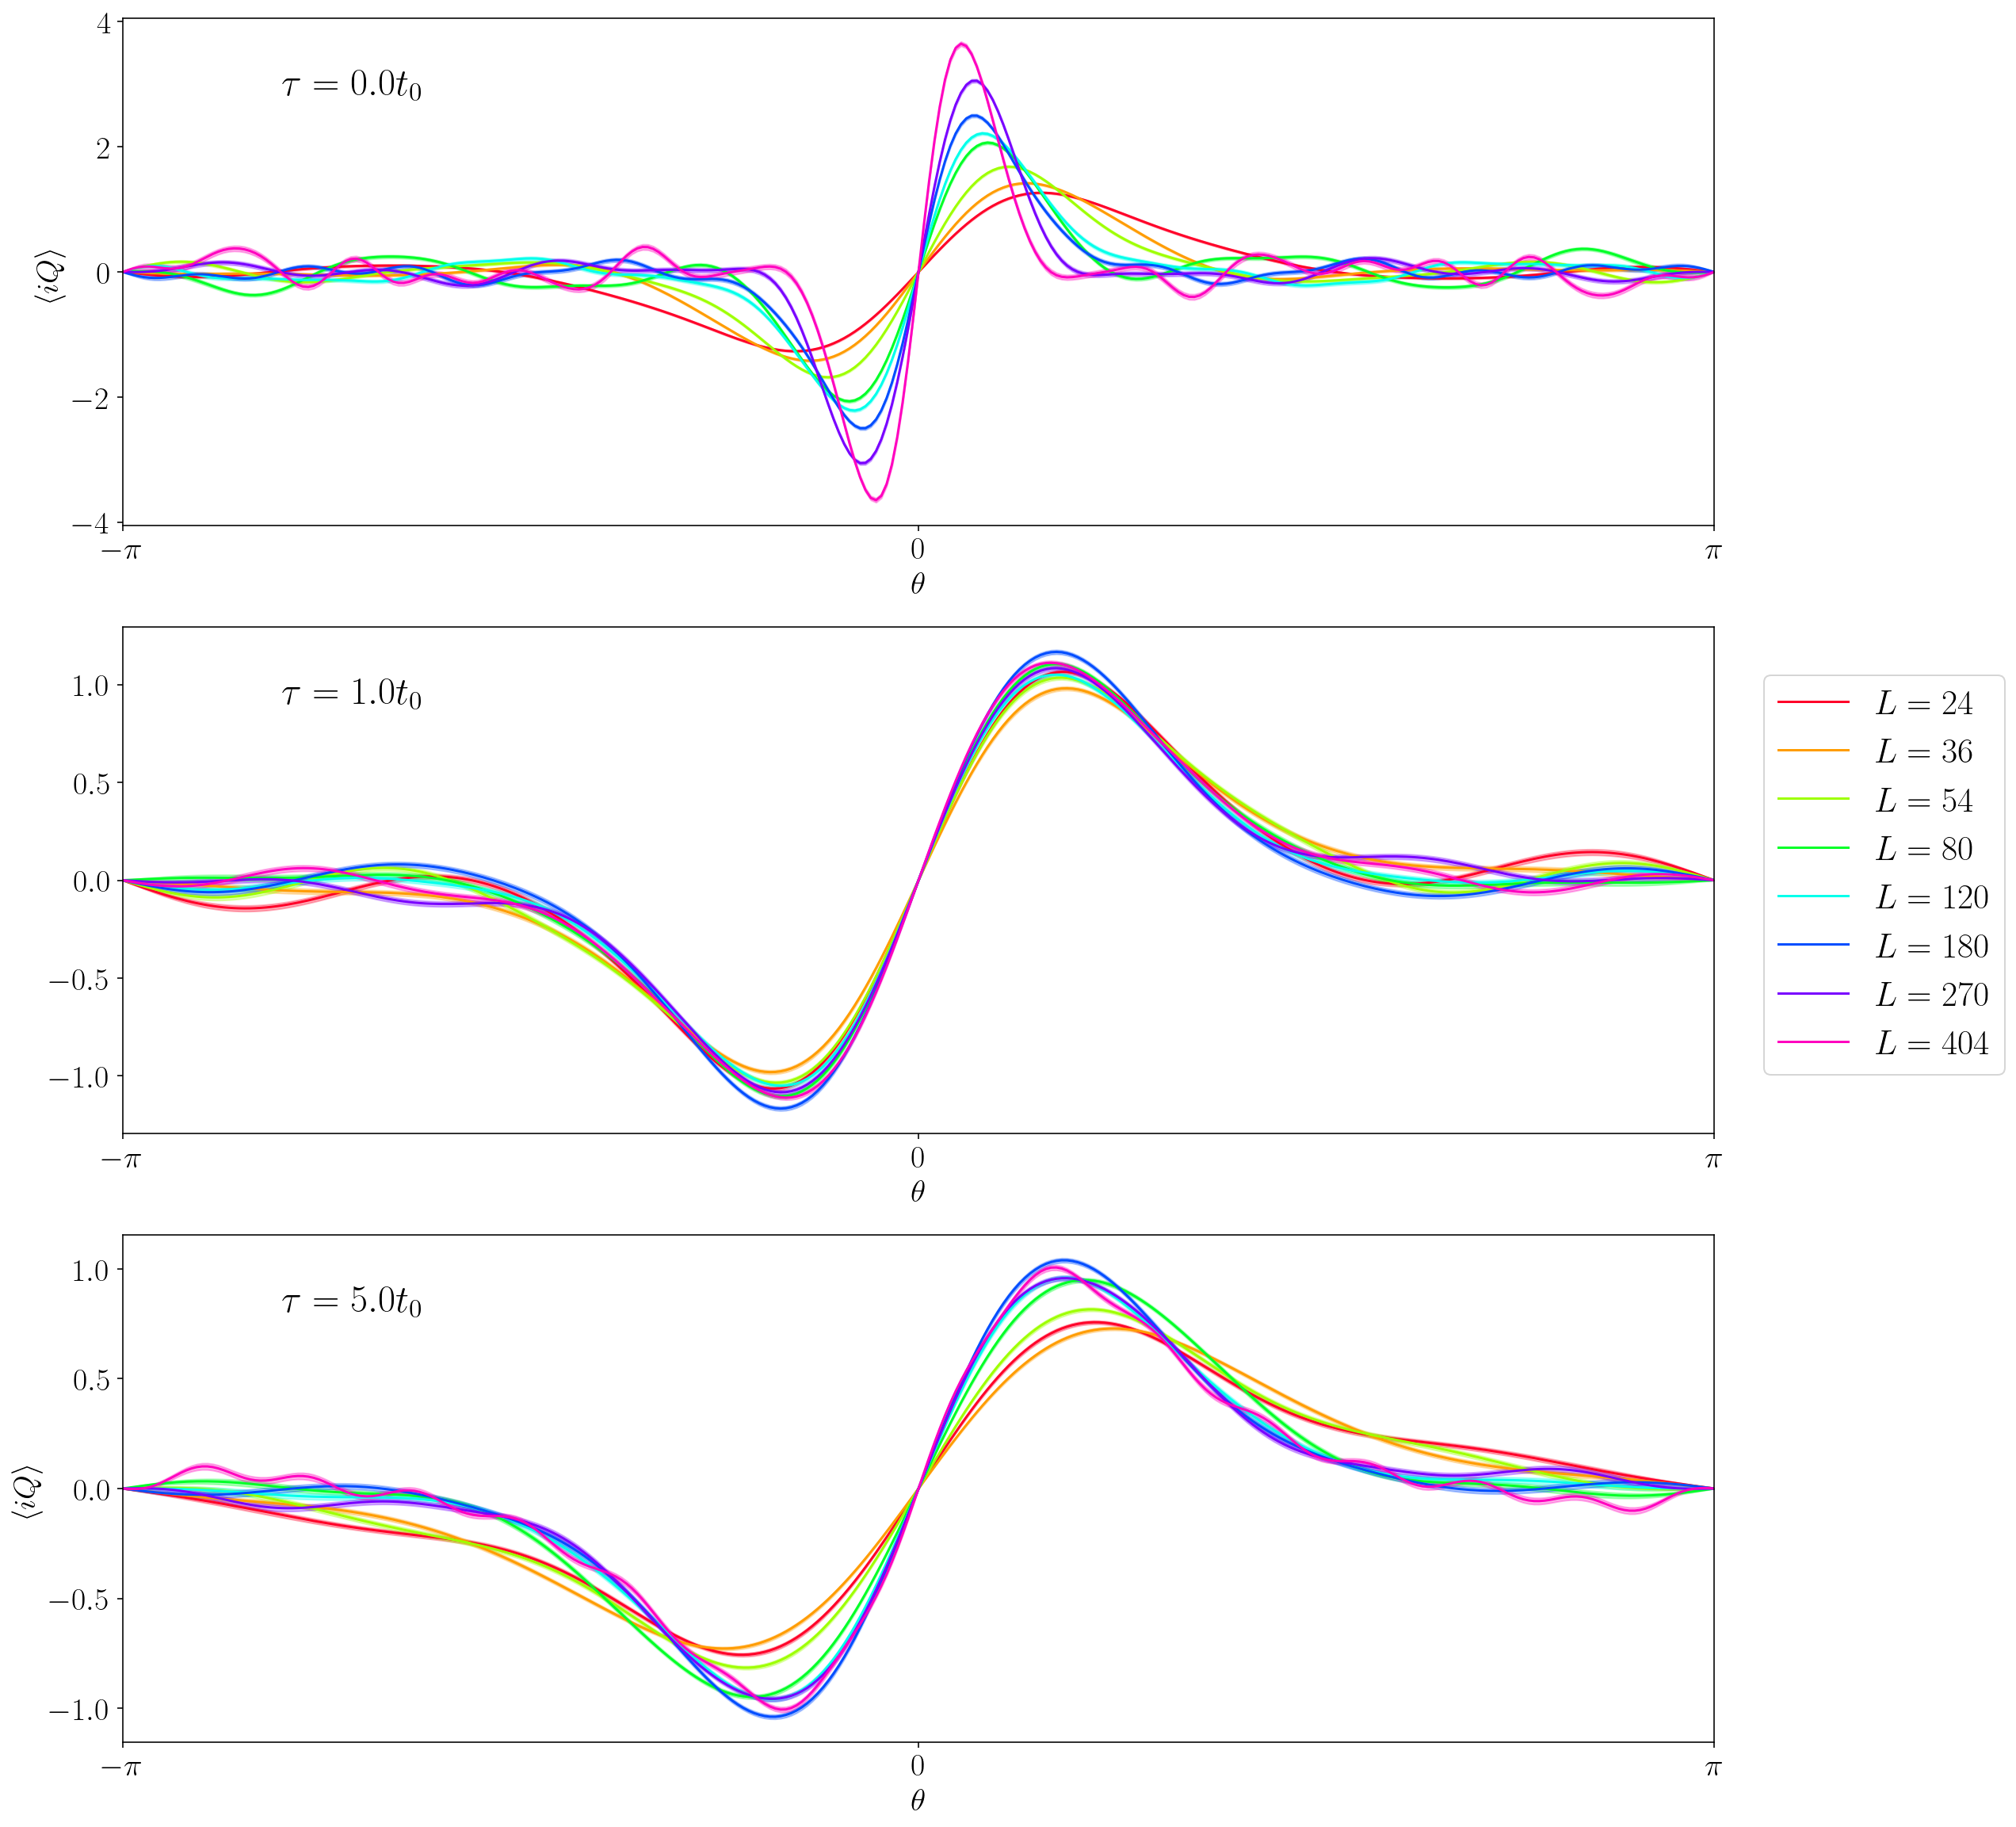
\includegraphics[width=\textwidth]{imgs/theta.png}
      \caption{\label{fig:theta} Imaginary part of $\langle Q \rangle$ as a function of $\theta$. Note the different scaling of the $y$-axis.}
\end{figure}


\begin{figure}[h]
    \centering
      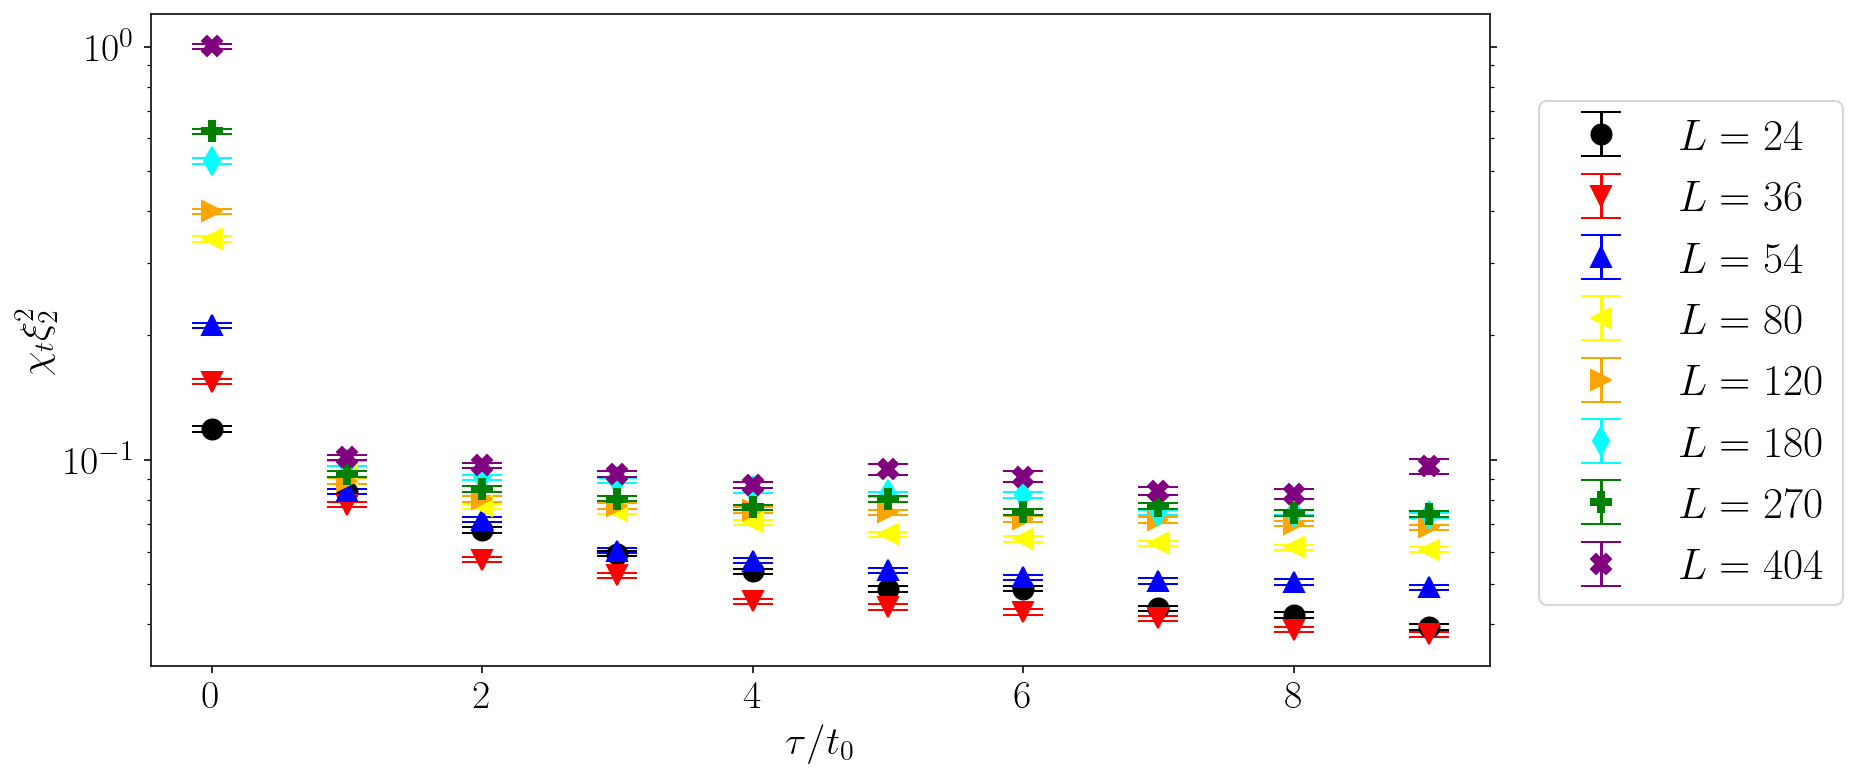
\includegraphics[width=\textwidth]{imgs/bietenholz.png}
      \caption{\label{fig:bietenholz} $\langle Q^2 \rangle=\chi_t L^2$ as a  }
\end{figure}

\begin{figure}[h]
    \centering
      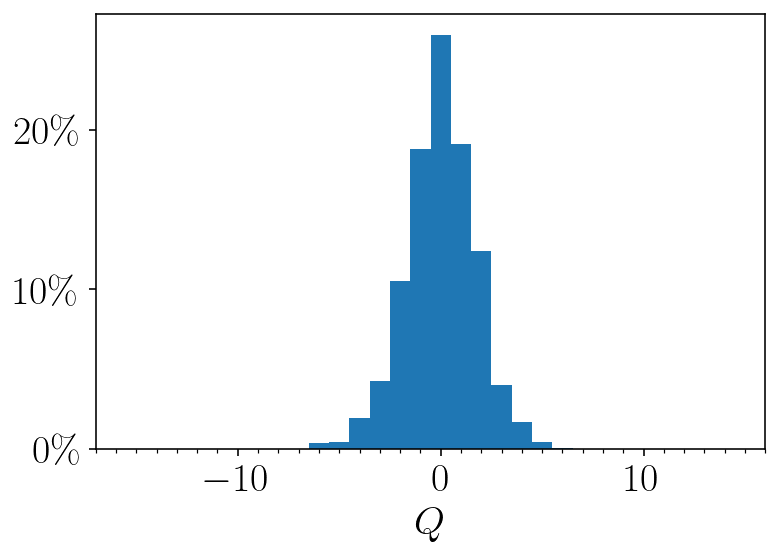
\includegraphics[width=0.6\textwidth]{imgs/hist.png}
      \caption{\label{fig:hist} Histogram of topological charge values $Q$ for trivial NLSM. $L=404$, 10,000 measurements, measurements very 50 sweps, 1,000 sweep thermalization, $\tau=0$}
\end{figure}




%\chapter{Statistical Analysis}

\chapter{Conclusion \& Outlook}


% MPI is unnecessary in this case


\appendix
\chapter{C++ NLSM Monte Carlo Program}
\lstset{language=C++,
                basicstyle=\scriptsize\ttfamily,
                keywordstyle=\color{blue}\ttfamily,
                stringstyle=\color{red}\ttfamily,
                commentstyle=\color{green}\ttfamily,
                morecomment=[l][\color{magenta}]{\#},
                breaklines=true,
                postbreak=\mbox{\textcolor{red}{$\hookrightarrow$}\space}
}

\codeexample{sweep.h}
\codeexample{sweep.cpp}
\codeexample{lattice.h}
\codeexample{lattice.cpp}
\codeexample{phi.h}
\codeexample{phi.cpp}
\codeexample{observables.h}
\codeexample{constants.h}

\bibliographystyle{unsrt}
\bibliography{library}

\end{document}
